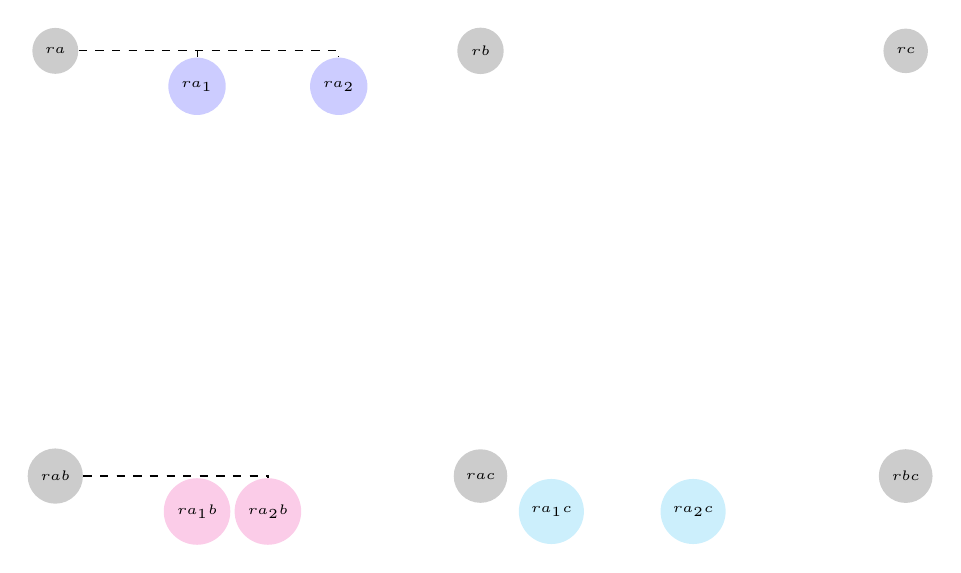
\begin{tikzpicture}
 [scale=1.8,auto=left,every node/.style={circle,fill=black!20,font=\tiny}]
  \node (na) at (0,8)  {$r a$};
  \node (na1)[fill=blue!20] at (1,7.75)  {$r a_1$};
  \node (na2)[fill=blue!20] at (2,7.75) {$r a_2$};
  \node (nb) at (3,8)  {$r b$};
  \node (nc) at (6,8)  {$r c$};
  \node (nab) at (0,5)  {$r a b$};
  \node (na1b)[fill=magenta!20] at (1.0,4.75)  {$r a_1 b$};
  \node (na2b)[fill=magenta!20] at (1.5,4.75)  {$r a_2 b$};
  \node (nac) at (3,5)  {$r a c$};
  \node (na1c)[fill=cyan!20] at (3.5,4.75)  {$r a_1 c$};
  \node (na2c)[fill=cyan!20] at (4.5,4.75)  {$r a_2 c$};
  \node (nbc) at (6,5)  {$r b c$};

  \foreach \from/\to in {na/na1,na/na2,nab/na1b,nab/na2b}
    \draw[dashed] (\from) -| (\to);


\end{tikzpicture}
